\documentclass[11pt,a4paper]{article}
\usepackage{amsmath}
\usepackage{amssymb}
\usepackage{geometry}
\usepackage{graphicx}
\usepackage{hyperref}
\usepackage{booktabs}
\usepackage{bm}
\usepackage{siunitx}
\usepackage{float}
\usepackage{tikz}
\usepackage{listings}
\usepackage{xcolor}
\usetikzlibrary{arrows.meta, positioning, shapes.geometric, calc, fit, backgrounds}

\geometry{margin=1in}

\definecolor{codegreen}{rgb}{0,0.6,0}
\definecolor{codegray}{rgb}{0.5,0.5,0.5}
\definecolor{codepurple}{rgb}{0.58,0,0.82}
\definecolor{backcolour}{rgb}{0.95,0.95,0.92}

\lstdefinestyle{mystyle}{
    backgroundcolor=\color{backcolour},
    commentstyle=\color{codegreen},
    keywordstyle=\color{magenta},
    numberstyle=\tiny\color{codegray},
    stringstyle=\color{codepurple},
    basicstyle=\ttfamily\footnotesize,
    breakatwhitespace=false,
    breaklines=true,
    captionpos=b,
    keepspaces=true,
    numbers=left,
    numbersep=5pt,
    showspaces=false,
    showstringspaces=false,
    showtabs=false,
    tabsize=2
}
\lstset{style=mystyle}

\title{3-DOF Vehicle Dynamics Implementation:\\
From 1-DOF to Full Planar Motion}
\author{Mario Tilocca}
\date{February 2026 -- Version 1.0}

\begin{document}

\maketitle

\begin{abstract}
This document describes the implementation of a full 3-DOF (longitudinal, lateral, yaw) vehicle dynamics model, extending the existing 1-DOF Dugoff-based tire model. We present the rigid body equations of motion, per-wheel kinematics accounting for vehicle rotation, coordinate frame transformations for steered wheels, and tire force sign conventions. The architecture integrates with a CAN-based control loop and explicit gear selector for forward/reverse operation.
\end{abstract}

\tableofcontents
\clearpage

%=============================================================================
\section*{Nomenclature}
%=============================================================================
\addcontentsline{toc}{section}{Nomenclature}

\begin{table}[H]
\centering
\begin{tabular}{lcl}
\toprule
\textbf{Symbol} & \textbf{Unit} & \textbf{Description} \\
\midrule
\multicolumn{3}{l}{\textit{Vehicle states}} \\
$v_x$            & \si{m/s}     & Longitudinal velocity (body frame) \\
$v_y$            & \si{m/s}     & Lateral velocity (body frame) \\
$\dot{\psi}$     & \si{rad/s}   & Yaw rate \\
$x, y$           & \si{m}       & Position (global frame) \\
$\psi$           & \si{rad}     & Heading / yaw angle \\
\midrule
\multicolumn{3}{l}{\textit{Tire / wheel quantities}} \\
$F_{x,i}$        & \si{N}       & Longitudinal tire force at wheel $i$ \\
$F_{y,i}$        & \si{N}       & Lateral tire force at wheel $i$ \\
$F_{z,i}$        & \si{N}       & Normal (vertical) load at wheel $i$ \\
$\omega_i$       & \si{rad/s}   & Wheel angular velocity \\
$\sigma_x$       & --           & Longitudinal slip ratio \\
$\sigma_y$       & --           & Lateral slip ratio (proxy for $\tan\alpha$) \\
$\alpha$         & \si{rad}     & Tire slip angle \\
$\lambda$        & --           & Friction utilization parameter (Dugoff) \\
$\delta$         & \si{rad}     & Wheel steer angle \\
\midrule
\multicolumn{3}{l}{\textit{Vehicle parameters}} \\
$m$              & \si{kg}      & Vehicle mass \\
$I_z$            & \si{kg.m^2}  & Yaw moment of inertia \\
$x_f, x_r$      & \si{m}       & CG distance to front / rear axle \\
$L$              & \si{m}       & Wheelbase ($x_f + x_r$) \\
$w$              & \si{m}       & Track width \\
$h_{\text{CG}}$  & \si{m}       & CG height above ground \\
$R$              & \si{m}       & Tire effective radius \\
$I_w$            & \si{kg.m^2}  & Wheel rotational inertia \\
\midrule
\multicolumn{3}{l}{\textit{Tire model parameters}} \\
$C_x$            & \si{N}       & Longitudinal slip stiffness \\
$C_y$            & \si{N}       & Lateral (cornering) stiffness \\
$\mu$            & --           & Surface friction coefficient \\
$g_{\text{dir}}$ & --           & Gear direction ($+1$, $-1$, or $0$) \\
$v_{\min}$       & \si{m/s}     & Low-speed regularisation threshold \\
\bottomrule
\end{tabular}
\caption{Principal symbols used in this document.}
\end{table}

\clearpage

%=============================================================================
\section{Introduction}
%=============================================================================

\subsection{From 1-DOF to 3-DOF}

The base vehicle model (documented in the companion Dugoff tire model document) provides:
\begin{itemize}
    \item 1-DOF longitudinal dynamics with Dugoff tire forces
    \item Wheel rotational dynamics and slip ratio computation
    \item Normal load distribution with longitudinal load transfer
    \item Ackermann steering geometry for front wheels
\end{itemize}

This document extends the model to \textbf{full planar motion (3-DOF)}:
\begin{equation}
\text{State: } \bm{x} = [v_x, v_y, \dot{\psi}, x, y, \psi]^\top
\end{equation}
where:
\begin{itemize}
    \item $v_x$ = longitudinal velocity (body frame)
    \item $v_y$ = lateral velocity (body frame)
    \item $\dot{\psi}$ = yaw rate
    \item $x, y$ = position (global frame)
    \item $\psi$ = heading angle (yaw)
\end{itemize}

\subsection{Motivation}

1-DOF models cannot capture:
\begin{itemize}
    \item \textbf{Lateral dynamics:} Cornering forces, sideslip, understeer/oversteer
    \item \textbf{Yaw dynamics:} Vehicle rotation from steering and lateral tire forces
    \item \textbf{Combined slip:} Interaction between longitudinal and lateral forces
    \item \textbf{Maneuver testing:} Slalom, lane change, emergency avoidance
\end{itemize}

The 3-DOF model enables realistic testing of:
\begin{itemize}
    \item Path tracking controllers
    \item Stability control systems
    \item Emergency maneuvers (double lane change, moose test)
    \item Combined braking-steering scenarios
\end{itemize}

%=============================================================================
\section{Rigid Body Dynamics (3-DOF)}
%=============================================================================

\subsection{Equations of Motion}

The vehicle is modeled as a rigid body in the plane with three degrees of freedom. All velocities and accelerations are expressed in the \textbf{body-fixed frame} (origin at CG, x-axis forward, y-axis left).

\subsubsection{Longitudinal Dynamics}

\begin{equation}
m \dot{v}_x = F_{x,\text{total}} - F_{\text{drag}} - F_{\text{roll}} + m v_y \dot{\psi}
\label{eq:long_dynamics}
\end{equation}

where:
\begin{align}
F_{x,\text{total}} &= F_{x,fl} + F_{x,fr} + F_{x,rl} + F_{x,rr} \\
F_{\text{drag}} &= c_d v_x |v_x| \\
F_{\text{roll}} &= c_r \cdot \text{sgn}(v_x)
\end{align}

\textbf{Critical Note:} The term $m v_y \dot{\psi}$ is the \textbf{centrifugal force} arising from the rotating reference frame. It is often omitted in simplified models, leading to instability.

\subsubsection{Lateral Dynamics}

\begin{equation}
m \dot{v}_y = F_{y,\text{total}} - m v_x \dot{\psi}
\label{eq:lat_dynamics}
\end{equation}

where:
\begin{equation}
F_{y,\text{total}} = F_{y,fl} + F_{y,fr} + F_{y,rl} + F_{y,rr}
\end{equation}

The term $-m v_x \dot{\psi}$ is the \textbf{centripetal acceleration} in the body frame. This coupling between longitudinal and lateral dynamics is \textbf{essential for stability}.

\subsubsection{Yaw Dynamics}

\begin{equation}
I_z \ddot{\psi} = M_{z,\text{total}}
\label{eq:yaw_dynamics}
\end{equation}

where the yaw moment is computed from the cross product $\bm{r}_i \times \bm{F}_i$ for each wheel:

\begin{equation}
M_{z,\text{total}} = \sum_{i=1}^{4} (x_i F_{y,i} - y_i F_{x,i})
\label{eq:yaw_moment}
\end{equation}

with wheel positions:
\begin{align}
\text{Front left:} \quad &\bm{r}_{fl} = [x_f, +w/2]^\top \\
\text{Front right:} \quad &\bm{r}_{fr} = [x_f, -w/2]^\top \\
\text{Rear left:} \quad &\bm{r}_{rl} = [-x_r, +w/2]^\top \\
\text{Rear right:} \quad &\bm{r}_{rr} = [-x_r, -w/2]^\top
\end{align}

where $x_f$ is CG distance to front axle, $x_r$ is CG distance to rear axle, and $w$ is track width.

\subsection{Position Integration}

Vehicle position in the global frame is computed by transforming body velocities:

\begin{align}
\dot{x} &= v_x \cos\psi - v_y \sin\psi \\
\dot{y} &= v_x \sin\psi + v_y \cos\psi \\
\dot{\psi} &= \dot{\psi}
\end{align}

This is a standard 2D rotation matrix $R(\psi)$ applied to $[v_x, v_y]^\top$.

%=============================================================================
\section{Per-Wheel Kinematics}
%=============================================================================

\subsection{Velocity at Wheel Center}

Each wheel experiences a different velocity due to:
\begin{enumerate}
    \item CG lateral velocity $v_y$
    \item Yaw rate $\dot{\psi}$ causing tangential velocity at offset from CG
\end{enumerate}

The velocity at wheel $i$ in the \textbf{vehicle frame} is:
\begin{equation}
\bm{v}_i = \begin{bmatrix} v_x \\ v_y \end{bmatrix} + \begin{bmatrix} -\dot{\psi} y_i \\ \dot{\psi} x_i \end{bmatrix} = \begin{bmatrix} v_x - \dot{\psi} y_i \\ v_y + \dot{\psi} x_i \end{bmatrix}
\end{equation}

For steered wheels (front), we must transform this to the \textbf{wheel frame} (aligned with wheel heading):

\begin{equation}
\begin{bmatrix} v_{x,w} \\ v_{y,w} \end{bmatrix} = \begin{bmatrix} \cos\delta & \sin\delta \\ -\sin\delta & \cos\delta \end{bmatrix} \begin{bmatrix} v_x - \dot{\psi} y_i \\ v_y + \dot{\psi} x_i \end{bmatrix}
\end{equation}

where $\delta$ is the wheel steer angle.

\subsection{Slip Angle Computation}

The slip angle $\alpha$ is the angle between the wheel heading and its velocity direction:

\begin{equation}
\alpha = \arctan\left(\frac{v_{y,w}}{|v_{x,w}|}\right)
\end{equation}

Note: We use $|v_{x,w}|$ (absolute value) to handle both forward and reverse motion correctly.

%=============================================================================
\section{Tire Force Coordinate Transformations}
%=============================================================================

\subsection{Rotation Matrix for Steered Wheels}

The Dugoff tire model computes forces $[F_x, F_y]^\top$ in the \textbf{wheel coordinate frame} (aligned with the wheel's heading). For steered wheels, these forces must be transformed to the \textbf{vehicle frame} before summing.

The standard 2D rotation matrix to express a wheel-frame vector in vehicle-frame coordinates is:

\begin{equation}
\begin{bmatrix} F_{x,veh} \\ F_{y,veh} \end{bmatrix} = \begin{bmatrix} \cos\delta & -\sin\delta \\ \sin\delta & \cos\delta \end{bmatrix} \begin{bmatrix} F_{x,wheel} \\ F_{y,wheel} \end{bmatrix}
\label{eq:rotation_matrix}
\end{equation}

Expanding:
\begin{align}
F_{x,veh} &= F_{x,wheel} \cos\delta - F_{y,wheel} \sin\delta \\
F_{y,veh} &= F_{x,wheel} \sin\delta + F_{y,wheel} \cos\delta
\end{align}

\textbf{Physical interpretation:} When the wheel is steered left ($\delta > 0$) and experiences a leftward force ($F_{y,wheel} > 0$), the transformation correctly produces a leftward force component in the vehicle frame, contributing to the intended turn direction.

%=============================================================================
\section{Tire Force Sign Conventions}
%=============================================================================

\subsection{Fundamental Principle}

Tire forces must \textbf{oppose slip} in all directions. This is the essence of friction.

\subsection{Longitudinal Force}

\subsubsection{Slip Ratio Definition}

\begin{equation}
\sigma_x = \frac{\omega R - V_x}{\max(|V_x|, |\omega R|, v_{\min})}
\end{equation}

Note: Denominator uses $|V_x|$ to prevent division by zero and handle reverse motion correctly.

\subsubsection{Force Formula with Gear Direction}

\begin{equation}
F_x = -g_{\text{dir}} \cdot C_x \sigma_x f(\lambda)
\label{eq:fx_formula}
\end{equation}

where $g_{\text{dir}}$ is the \textbf{gear direction} from CAN command:
\begin{itemize}
    \item Forward: $g_{\text{dir}} = +1$
    \item Reverse: $g_{\text{dir}} = -1$
    \item Neutral: $g_{\text{dir}} = 0$
\end{itemize}

\textbf{Physical interpretation:}
\begin{itemize}
    \item Forward gear, $\sigma_x > 0$ (wheel spinning faster): $F_x < 0$ (brakes vehicle)
    \item Forward gear, $\sigma_x < 0$ (wheel locked): $F_x > 0$ (resists locking, ABS effect)
    \item Reverse gear, $\sigma_x > 0$: $F_x > 0$ (resists reverse motion)
    \item Neutral: $F_x = 0$ (no longitudinal traction)
\end{itemize}

\subsection{Lateral Force}

\begin{equation}
F_y = -C_y \sigma_y f(\lambda)
\end{equation}

where $\sigma_y = V_y / |V_x|$ is the lateral slip ratio (small-angle approximation of slip angle).

Lateral force is \textbf{independent} of gear direction. It always opposes lateral slip regardless of forward/reverse motion. The negative sign ensures the force resists slip: if the wheel slips left ($\sigma_y > 0$), the force pushes right ($F_y < 0$).

%=============================================================================
\section{Dugoff Tire Model Summary}
%=============================================================================

This section provides a self-contained summary of the Dugoff tire model used to compute $F_{x,i}$ and $F_{y,i}$. A full derivation is given in the companion document~\cite{dugoff_doc}.

\subsection{Fundamental Equations}

The Dugoff model computes tire forces as the product of a linear slip stiffness, the slip ratio, and a nonlinear saturation function:

\begin{align}
F_x &= -g_{\text{dir}} \cdot C_x \sigma_x \, f(\lambda) \\
F_y &= -C_y \sigma_y \, f(\lambda)
\end{align}

The sign conventions are detailed in Section~5. The negative signs ensure forces oppose slip.

\subsection{Friction Utilisation Parameter}

The parameter $\lambda$ measures how close the tyre is to its friction limit:

\begin{equation}
\lambda = \frac{\mu F_z}{2\sqrt{(C_x \sigma_x)^2 + (C_y \sigma_y)^2}}
\end{equation}

When $\lambda \geq 1$ the tyre operates in the \emph{linear} (grip-available) regime; when $\lambda < 1$ the available friction is exceeded and forces saturate.

\subsection{Saturation Function}

\begin{equation}
f(\lambda) = \begin{cases}
(2 - \lambda)\lambda, & \lambda < 1 \quad \text{(saturated / sliding)} \\
1,                     & \lambda \geq 1 \quad \text{(linear / grip available)}
\end{cases}
\end{equation}

This function is continuous at $\lambda=1$ and smoothly reduces the force magnitude as the friction circle is approached. It guarantees the resultant tyre force never exceeds $\mu F_z$:

\begin{equation}
\sqrt{F_x^2 + F_y^2} \leq \mu F_z
\end{equation}

\subsection{Load-Dependent Stiffness}

Slip stiffness scales linearly with normal load:

\begin{align}
C_x(F_z) &= C_{x,\text{base}} \cdot \frac{F_z}{F_{z,\text{ref}}} \\[4pt]
C_y(F_z) &= C_{y,\text{base}} \cdot \frac{F_z}{F_{z,\text{ref}}}
\end{align}

where $F_{z,\text{ref}}$ is a reference load (typically one-quarter static weight). This coupling means load transfer during braking or cornering directly affects available grip at each wheel.

\subsection{Wheel Rotational Dynamics}

Each wheel integrates angular velocity from the net torque:

\begin{equation}
I_w \dot{\omega}_i = \tau_{\text{drive},i} - \tau_{\text{brake},i} - F_{x,i} R
\label{eq:wheel_dynamics}
\end{equation}

The feedback term $-F_{x,i} R$ couples the tyre force back into wheel speed, enabling natural slip development, wheel spin under excess drive torque, and wheel lock under heavy braking.

%=============================================================================
\section{Yaw Moment Calculation}
%=============================================================================

\subsection{Cross Product Formula}

For a force $\bm{F} = [F_x, F_y]^\top$ at position $\bm{r} = [x, y]^\top$ relative to the CG, the yaw moment (z-component of $\bm{r} \times \bm{F}$) is:

\begin{equation}
M_z = x F_y - y F_x
\label{eq:cross_product}
\end{equation}

\textbf{Physical example:} A leftward force ($F_y > 0$) at the front-left wheel with position $(x_f > 0, y > 0)$ creates:
\begin{equation}
M_z = x_f F_y - y \cdot 0 = x_f F_y > 0 \quad \text{(CCW yaw, left turn)}
\end{equation}

This is correct: a left force on the left side of the vehicle creates a left (counterclockwise) turn.

%=============================================================================
\section{Centripetal Coupling in Rotating Reference Frame}
%=============================================================================

\subsection{Equations in Body Frame}

In the vehicle body frame (rotating with the vehicle), both longitudinal and lateral velocities are affected by rotation:

\begin{align}
\dot{v}_x &= \frac{F_x}{m} + v_y \dot{\psi} \quad &\text{(centrifugal acceleration)} \\
\dot{v}_y &= \frac{F_y}{m} - v_x \dot{\psi} \quad &\text{(centripetal acceleration)}
\end{align}

The terms $v_y \dot{\psi}$ and $-v_x \dot{\psi}$ arise from the non-inertial (rotating) reference frame. They are \textbf{essential for stability} and must be included in the integration.

\subsection{Physical Interpretation}

When the vehicle turns (yaw rate $\dot{\psi} \neq 0$):
\begin{itemize}
    \item \textbf{Centrifugal effect} ($v_y \dot{\psi}$): Lateral velocity creates an apparent longitudinal acceleration in the body frame
    \item \textbf{Centripetal effect} ($-v_x \dot{\psi}$): Longitudinal velocity requires centripetal acceleration to maintain circular motion
\end{itemize}

These terms couple the longitudinal and lateral dynamics, making the 3-DOF model fundamentally different from independent 1-DOF models.

%=============================================================================
\section{CAN-Based Control Architecture}
%=============================================================================

\subsection{Gear Selector Implementation}

To properly handle forward/reverse motion, an explicit \textbf{gear selector} was implemented via CAN (matching real autonomous vehicle architecture).

\subsubsection{CAN Signal Definition}

Frame: \texttt{ACTUATOR\_CMD\_1} (0x100), 10 ms cycle

\begin{table}[H]
\centering
\begin{tabular}{lcccl}
\toprule
\textbf{Signal} & \textbf{Start Bit} & \textbf{Length} & \textbf{Values} & \textbf{Unit} \\
\midrule
system\_enable & 0 & 1 & 0/1 & bool \\
gear\_position & 1 & 2 & 0--3 & enum \\
mode & 3 & 2 & 0--3 & enum \\
steer\_cmd\_deg & 8 & 16 & -500..500 & deg \\
drive\_torque\_cmd\_nm & 24 & 16 & -300k..300k & Nm \\
brake\_cmd\_pct & 40 & 8 & 0..100 & \% \\
\bottomrule
\end{tabular}
\caption{CAN actuator command signals}
\end{table}

Gear position encoding:
\begin{itemize}
    \item 0 = Neutral (no longitudinal force)
    \item 1 = Forward (default)
    \item 2 = Reverse
    \item 3 = Reserved
\end{itemize}

\subsubsection{Data Flow}

\begin{equation}
\text{CAN} \to \text{ActuatorCmd} \to \text{PlantState} \to \text{WheelSubsystem} \to \text{Dugoff}(g_{\text{dir}})
\end{equation}

The gear position is:
\begin{enumerate}
    \item Decoded from CAN frame (bits 1--2)
    \item Stored in \texttt{ActuatorCmd.gear\_position}
    \item Copied to \texttt{PlantState.gear\_position} by \texttt{PlantModel}
    \item Converted to direction integer by \texttt{WheelSubsystem}
    \item Passed to \texttt{TyreDugoff::compute\_forces()} as parameter
\end{enumerate}

\subsection{Subsystem Execution Order}

The plant model uses a \textbf{priority-ordered subsystem manager}:

\begin{table}[H]
\centering
\begin{tabular}{clll}
\toprule
\textbf{Priority} & \textbf{Subsystem} & \textbf{Inputs} & \textbf{Outputs} \\
\midrule
50  & Steer & $\delta_{\text{cmd}}$ & $\delta_{fl}, \delta_{fr}$ \\
100 & Drive & $\tau_{\text{cmd}}, \text{brake}_{\%}$ & $\tau_{\text{drive},i}, \tau_{\text{brake},i}$ \\
105 & Wheel & $\tau_{i}, v_x, v_y, \dot{\psi}$ & $F_{x,i}, F_{y,i}, \omega_i$ \\
110 & Vehicle & $F_{x,i}, F_{y,i}$ & $v_x, v_y, \dot{\psi}, x, y, \psi$ \\
150 & Battery & $P_{\text{elec}}$ & SOC, $V$, $I$ \\
\bottomrule
\end{tabular}
\caption{Subsystem execution order}
\end{table}

Lower priority numbers execute first, ensuring correct data dependencies.

%=============================================================================
\section{System Block Diagram}
%=============================================================================

\begin{figure}[H]
\centering
\resizebox{\textwidth}{!}{%
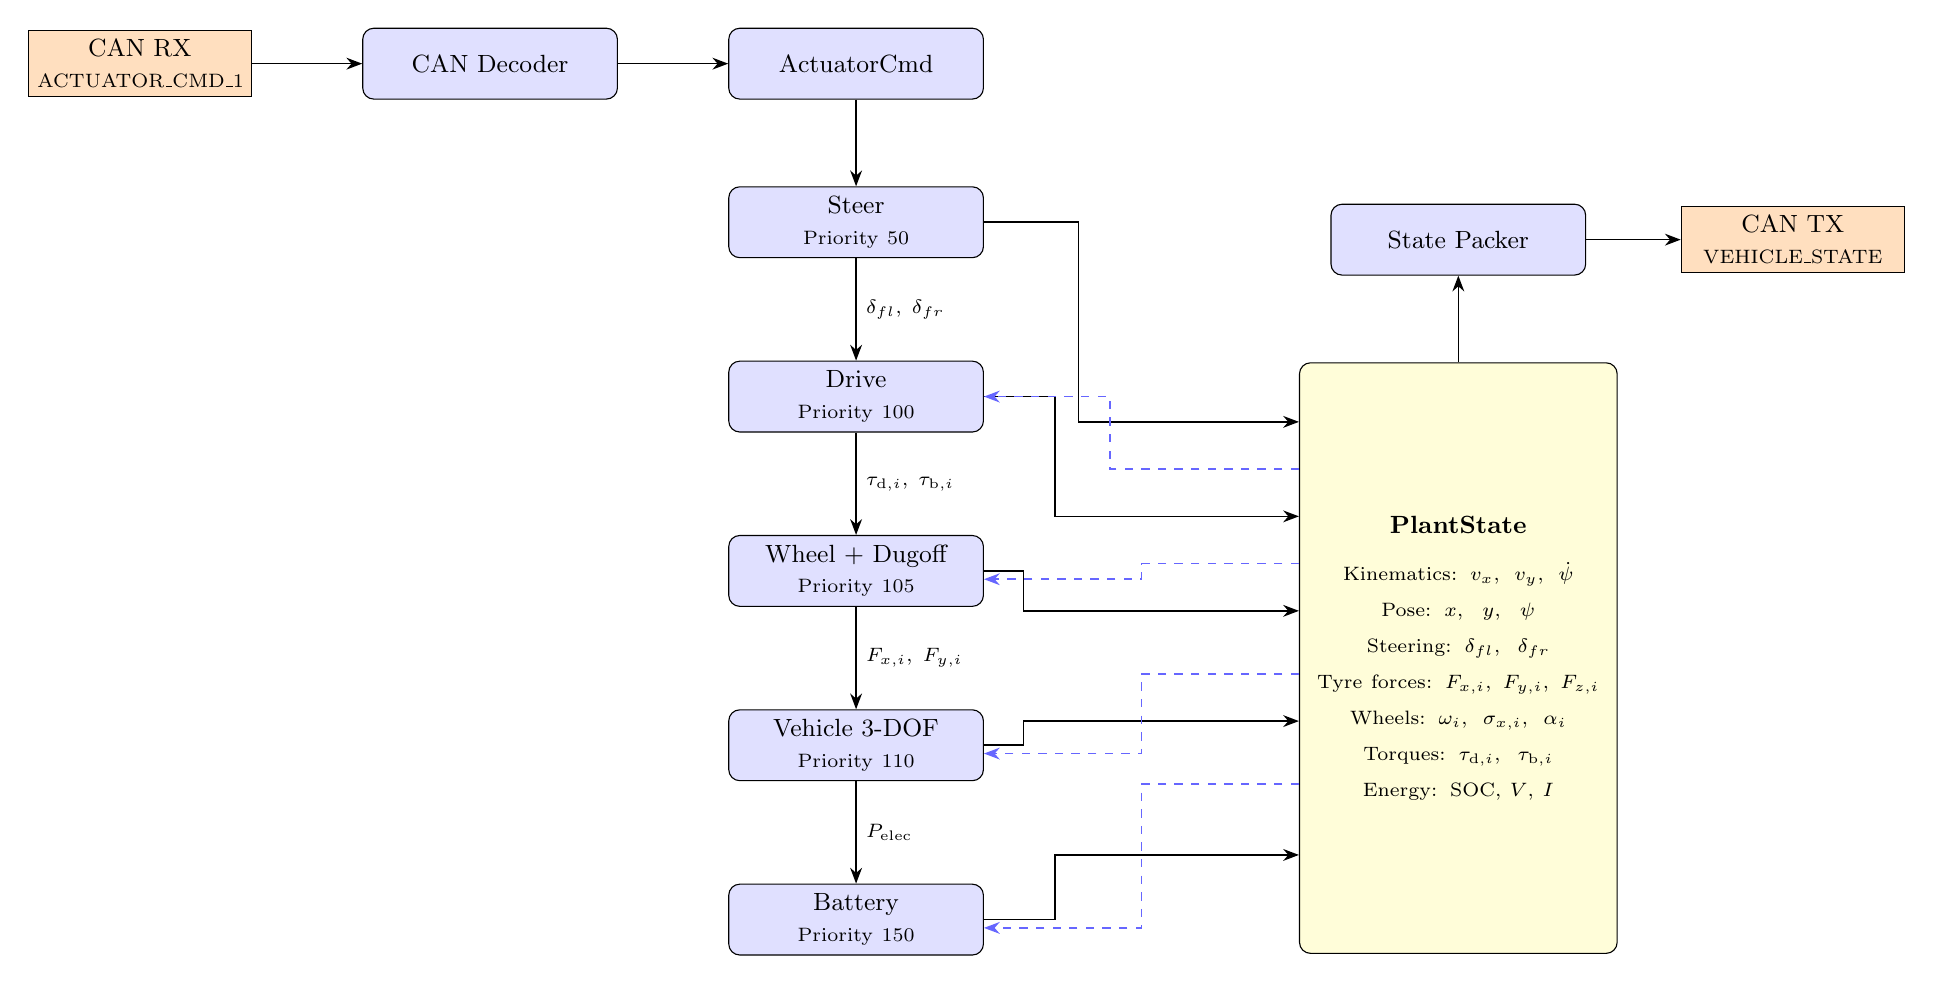
\begin{tikzpicture}[
    node distance=1.3cm and 1.4cm,
    block/.style={rectangle, draw, fill=blue!12, text width=3cm,
                  text centered, rounded corners, minimum height=0.9cm, font=\small},
    can/.style={rectangle, draw, fill=orange!25, text width=2.6cm,
                text centered, minimum height=0.8cm, font=\small},
    state/.style={rectangle, draw, fill=yellow!15, text width=3.8cm,
                  text centered, rounded corners, minimum height=7.5cm, font=\small},
    arrow/.style={-Stealth, semithick},
    fb/.style={-Stealth, semithick, dashed, blue!60}
]

% ---- Top row: CAN RX path ----
\node[can] (canrx) {CAN RX\\{\scriptsize ACTUATOR\_CMD\_1}};
\node[block, right=of canrx] (decoder) {CAN Decoder};
\node[block, right=of decoder] (actcmd) {ActuatorCmd};

% ---- Subsystem cascade (left column) ----
\node[block, below=1.1cm of actcmd] (steer)   {Steer\\{\scriptsize Priority 50}};
\node[block, below=of steer]        (drive)   {Drive\\{\scriptsize Priority 100}};
\node[block, below=of drive]        (wheel)   {Wheel + Dugoff\\{\scriptsize Priority 105}};
\node[block, below=of wheel]        (vehicle) {Vehicle 3-DOF\\{\scriptsize Priority 110}};
\node[block, below=of vehicle]      (battery) {Battery\\{\scriptsize Priority 150}};

% ---- PlantState (right column, vertically centered) ----
\coordinate (mid) at ($(wheel.east)!0.5!(vehicle.east)$);
\node[state, right=4.0cm of mid] (ps) {
    \textbf{PlantState}\\[6pt]
    {\scriptsize Kinematics: $v_x,\; v_y,\; \dot{\psi}$}\\[2pt]
    {\scriptsize Pose: $x,\; y,\; \psi$}\\[2pt]
    {\scriptsize Steering: $\delta_{fl},\; \delta_{fr}$}\\[2pt]
    {\scriptsize Tyre forces: $F_{x,i},\; F_{y,i},\; F_{z,i}$}\\[2pt]
    {\scriptsize Wheels: $\omega_i,\; \sigma_{x,i},\; \alpha_i$}\\[2pt]
    {\scriptsize Torques: $\tau_{\text{d},i},\; \tau_{\text{b},i}$}\\[2pt]
    {\scriptsize Energy: SOC, $V$, $I$}
};

% ---- Top-right: CAN TX path ----
\node[block, above=1.1cm of ps] (packer) {State Packer};
\node[can, right=1.2cm of packer] (cantx) {CAN TX\\{\scriptsize VEHICLE\_STATE}};

% ======== Forward flow ========
\draw[arrow] (canrx) -- (decoder);
\draw[arrow] (decoder) -- (actcmd);
\draw[arrow] (actcmd) -- (steer);

% ======== Subsystem cascade ========
\draw[arrow] (steer)   -- node[right, font=\scriptsize]{$\delta_{fl},\;\delta_{fr}$} (drive);
\draw[arrow] (drive)   -- node[right, font=\scriptsize]{$\tau_{\text{d},i},\;\tau_{\text{b},i}$} (wheel);
\draw[arrow] (wheel)   -- node[right, font=\scriptsize]{$F_{x,i},\;F_{y,i}$} (vehicle);
\draw[arrow] (vehicle) -- node[right, font=\scriptsize]{$P_{\text{elec}}$} (battery);

% ======== Write-back: subsystem → PlantState (solid) ========
% Staggered entry points on ps.west; vertical segments near subsystem column
\draw[arrow] (steer.east)   -- ++(1.2,0) |- ([yshift= 3.0cm]ps.west);
\draw[arrow] (drive.east)   -- ++(0.9,0) |- ([yshift= 1.8cm]ps.west);
\draw[arrow] (wheel.east)   -- ++(0.5,0) |- ([yshift= 0.6cm]ps.west);
\draw[arrow] (vehicle.east) -- ++(0.5,0) |- ([yshift=-0.8cm]ps.west);
\draw[arrow] (battery.east) -- ++(0.9,0) |- ([yshift=-2.5cm]ps.west);

% ======== Feedback: PlantState → subsystem (dashed blue) ========
% Staggered exit points on ps.west; vertical segments near PlantState column
\draw[fb] ([yshift= 2.4cm]ps.west) -- ++(-2.4,0) |- (drive.east);
\draw[fb] ([yshift= 1.2cm]ps.west) -- ++(-2.0,0) |- ([yshift=-3pt]wheel.east);
\draw[fb] ([yshift=-0.2cm]ps.west) -- ++(-2.0,0) |- ([yshift=-3pt]vehicle.east);
\draw[fb] ([yshift=-1.6cm]ps.west) -- ++(-2.0,0) |- ([yshift=-3pt]battery.east);

% ======== CAN output flow ========
\draw[arrow] (ps) -- (packer);
\draw[arrow] (packer) -- (cantx);

\end{tikzpicture}
}% end resizebox
\caption{3-DOF plant model architecture with CAN-based closed-loop control.
Subsystems execute in priority order (lower number $=$ first).
Solid arrows denote write-back into the shared \texttt{PlantState};
dashed blue arrows denote feedback reads.
The CAN TX path packs selected state variables for the external controller.}
\end{figure}


%=============================================================================
\section{Load Transfer (Longitudinal and Lateral)}
%=============================================================================

The normal loads $F_{z,i}$ at each wheel vary due to:
\begin{enumerate}
    \item Static weight distribution
    \item Longitudinal load transfer during acceleration/braking
    \item Lateral load transfer during cornering
\end{enumerate}

\subsection{Static Load Distribution}

\begin{align}
F_{z,fl}^{\text{static}} &= F_{z,fr}^{\text{static}} = \frac{mg}{2} \frac{x_r}{L} \\
F_{z,rl}^{\text{static}} &= F_{z,rr}^{\text{static}} = \frac{mg}{2} \frac{x_f}{L}
\end{align}

where $L = x_f + x_r$ is the wheelbase.

\subsection{Longitudinal Load Transfer}

\begin{align}
\Delta F_{z,\text{front}} &= \frac{m a_x h_{\text{CG}}}{L} \\
\Delta F_{z,\text{rear}} &= -\frac{m a_x h_{\text{CG}}}{L}
\end{align}

where $h_{\text{CG}}$ is the CG height above ground.

\subsection{Lateral Load Transfer}

Within each axle:
\begin{align}
\Delta F_{z,\text{left}} &= -\frac{m a_y h_{\text{CG}}}{w} \\
\Delta F_{z,\text{right}} &= +\frac{m a_y h_{\text{CG}}}{w}
\end{align}

where $w$ is the track width.

\subsection{Combined Normal Loads}

\begin{align}
F_{z,fl} &= F_{z,fl}^{\text{static}} + \Delta F_{z,\text{front}} + \Delta F_{z,\text{left}} \\
F_{z,fr} &= F_{z,fr}^{\text{static}} + \Delta F_{z,\text{front}} + \Delta F_{z,\text{right}} \\
F_{z,rl} &= F_{z,rl}^{\text{static}} + \Delta F_{z,\text{rear}} + \Delta F_{z,\text{left}} \\
F_{z,rr} &= F_{z,rr}^{\text{static}} + \Delta F_{z,\text{rear}} + \Delta F_{z,\text{right}}
\end{align}

%=============================================================================
\section{Validation}
%=============================================================================

The 3-DOF model was validated through:

\begin{enumerate}
    \item \textbf{Slalom maneuver:} $\pm 5°$ steering at 17 m/s
    \begin{itemize}
        \item Lateral velocity remained $< 0.03$ m/s
        \item Sideslip angle $< 180°$ (within typical limits)
        \item Yaw rate response proportional to steering input
    \end{itemize}

    \item \textbf{Coast-down test:} Zero torque from 15 m/s
    \begin{itemize}
        \item Consistent negative acceleration from drag
        \item No oscillations or positive acceleration spikes
        \item Vehicle decelerated smoothly to rest
    \end{itemize}

    \item \textbf{Emergency stop:} Full braking from 17 m/s
    \begin{itemize}
        \item All wheels maintained slip ratio $< 0.95$
        \item Friction utilization $\lambda \approx 1$ (saturated)
        \item No wheel lock (ABS-like behavior from Dugoff saturation)
    \end{itemize}
\end{enumerate}

%=============================================================================
\section{Conclusion}
%=============================================================================

This document presented the implementation of a full 3-DOF vehicle dynamics model extending the existing 1-DOF Dugoff tire model. The key contributions are:

\begin{itemize}
    \item Complete rigid body dynamics with centrifugal/centripetal coupling
    \item Per-wheel kinematics accounting for yaw rate and wheel positions
    \item Coordinate frame transformations for steered wheels
    \item Proper yaw moment calculation from tire forces
    \item CAN-based gear selector architecture
\end{itemize}

The model enables realistic simulation of lateral maneuvers, combined braking-steering scenarios, and stability analysis for autonomous mining haul trucks.

\subsection{Future Enhancements}

Potential extensions include:
\begin{itemize}
    \item Roll dynamics (4-DOF or 6-DOF model)
    \item Suspension compliance and tire vertical dynamics
    \item Road bank angle and grade effects
    \item Enhanced tire models (Pacejka MF, TameTire)
    \item Validation against real vehicle telemetry
\end{itemize}

%=============================================================================
% References
%=============================================================================
\begin{thebibliography}{9}
\bibitem{dugoff_doc}
M.~Tilocca,
\textit{Vehicle Dynamics, Battery, and Sensor Models (Dugoff Tire + Sensor Simulation)},
Version~2.1, January 2026.
\end{thebibliography}

\end{document}
